% --------------------------------------------------------------
% This is all preamble stuff that you don't have to worry about.
% Head down to where it says "Start here"
% --------------------------------------------------------------
 
\documentclass[12pt]{article}
 
\usepackage[margin=1in]{geometry} 
\usepackage{amsmath,amsthm,amssymb}
\usepackage{graphicx}
\newcommand{\N}{\mathbb{N}}
\newcommand{\Z}{\mathbb{Z}}
\usepackage{algorithmic}
\newenvironment{theorem}[2][Theorem]{\begin{trivlist}
\item[\hskip \labelsep {\bfseries #1}\hskip \labelsep {\bfseries #2.}]}{\end{trivlist}}
\newenvironment{lemma}[2][Lemma]{\begin{trivlist}
\item[\hskip \labelsep {\bfseries #1}\hskip \labelsep {\bfseries #2.}]}{\end{trivlist}}
\newenvironment{exercise}[2][Exercise]{\begin{trivlist}
\item[\hskip \labelsep {\bfseries #1}\hskip \labelsep {\bfseries #2.}]}{\end{trivlist}}
\newenvironment{reflection}[2][Reflection]{\begin{trivlist}
\item[\hskip \labelsep {\bfseries #1}\hskip \labelsep {\bfseries #2.}]}{\end{trivlist}}
\newenvironment{proposition}[2][Proposition]{\begin{trivlist}
\item[\hskip \labelsep {\bfseries #1}\hskip \labelsep {\bfseries #2.}]}{\end{trivlist}}
\newenvironment{corollary}[2][Corollary]{\begin{trivlist}                      
\item[\hskip \labelsep {\bfseries #1}\hskip \labelsep {\bfseries #2.}]}{\end{trivlist}}
\newenvironment{definition}[2][definition]{\begin{trivlist}                      
\item[\hskip \labelsep {\bfseries #1}\hskip \labelsep {\bfseries #2.}]}{\end{trivlist}}
 
\begin{document}
 
% --------------------------------------------------------------
%                         Start here
% --------------------------------------------------------------
 
%\renewcommand{\qedsymbol}{\filledbox}
 
\title{Homework \#6}%replace X with the appropriate number
\author{\\ %replace with your name
CPSC 395 - Analysis of Algorithms
\\ Due: Monday, 22} %if necessary, replace with your course title
\date{}
\maketitle

\begin{enumerate}
\item Exercise 9.1-1 (Drawing binary trees to picture the comparisons helps)\\
Show that the second smallest of n elements can be found with n + $\ceil{lgn}$ - 2 comparisons in the worst case. (Hint: Also find the smallest element.) \\

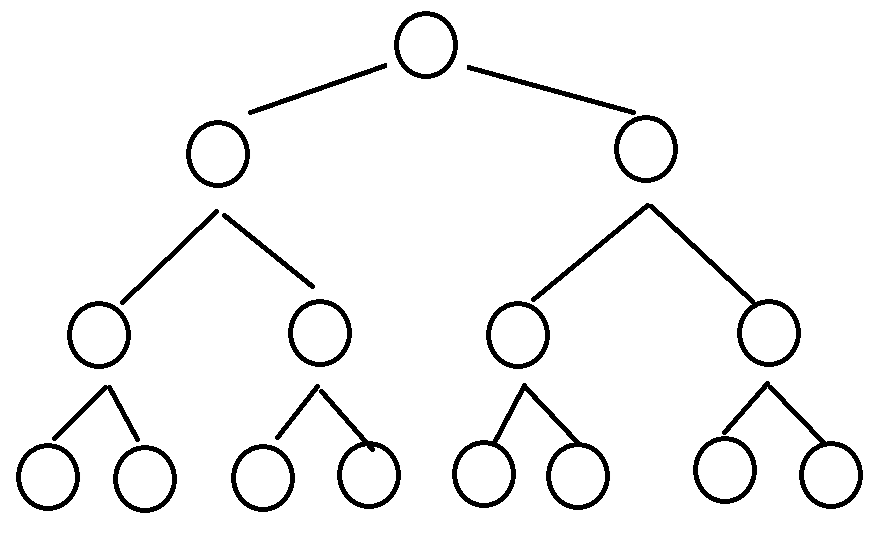
\includegraphics[scale=.25]{9.1.1.png} \\
As was described during our last class, the elements are compared in a tournament style. Pairs are compared and then the winners get compared and so on until there is a final "winner". The winner in this case is the smallest element. It takes n-1 comparisons to find the winner. The height to of a tree is lgn. So the process of finding the second smallest element would first require finding a winner, so that is already n-1 comparisons. The second smallest could be anywhere in the tree depending on when it was compared against the smallest, so in the worst case it would take lgn - 1 comparisons due to having to go all the way up to the level below the winner. n - 1 + lgn - 1 comparisons would be a total of n + lgn - 2 for the worst case.

\item Exercise 9.2-3 \\
Write an iterative version of RANDOMIZED-SELECT. \\
Here is the original version of RANDOMIZED-SELECT\\
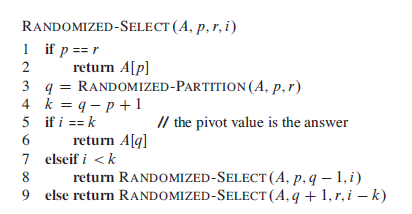
\includegraphics[scale=1]{Randomselect.png}
\\
For an iterative version, first we're gonna need to replace the recursive calls. We're going to need a loop to take the place of the recursive calls.

\begin{algorithmic}
\STATE RANDOMIZED-SELECT(A,p,r,i)
\WHILE{}
\IF{p == r}
\STATE return A[p]
\ENDIF
\STATE q = RANDOMIZED-PARTITION(A,p,r)
\STATE k = q - p + 1
\IF{i == k}
\STATE return A[q]
\ELSIF{i $<$ k}
\STATE r = q - 1
\ELSE
\STATE p = q + 1
\STATE i = i - k
\ENDIF
\ENDWHILE
\end{algorithmic}

\item Exercise 9.3-3 \\
Show how quicksort can be made to run in O(nlgn) time in the worst case, assuming
that all elements are distinct.\\

The typical worst case scenario of Quicksort is O($n^2)$. 


\item Exercise 9.3-5 \\
Suppose that you have a “black-box” worst-case linear-time median subroutine.
Give a simple, linear-time algorithm that solves the selection problem for an arbitrary
order statistic. \\

A black-box model is when you focus on the inputs and outputs while not knowing about the inner workings and assuming it does what is needed. 

\end{enumerate}
 
 
 Please email me if you have any questions.

% --------------------------------------------------------------
%     You don't have to mess with anything below this line.
% --------------------------------------------------------------
 
\end{document}